\chapter{الطفرات وتنويع المورثوم}\label{ch:b2:genome-diversification}

انثر مليار بكتيريا على طبق مطعّم بصادّ، فتجد في صباح اليوم التالي
حفنة من المستعمرات قد نمت. فهل علّم الدواء تلك الخلايا أن تقاومه، أم
كانت مقاومة قبل أن تلقاه؟ يبدو السؤال فلسفيًا، وقد حسمته تجربة
بالغة الأناقة سنة 1943: فالخلايا المقاومة كانت موجودة سلفًا، أنتجتها
طفرات وقعت عشوائيًا، دون اعتبار لنفعها. وهذا الفصل عن مصادر ذلك
التنوع --- أخطاء النسخ، والحوادث الكيميائية، والمورّثات \omterm{def:b2:genome-diversification:transposon}{القافزة}،
والمورّثات المتبادلة بين الخلايا، ومضاعفات المورّثات والمورثومات
كلها --- وعن السرعة التي تجري بها. أما الانتخاب الذي يفرز هذا
التنوع فموضوع \cref{ch:b2:population-genetics}؛ والموضوع هنا هو من
أين تأتي المادة الخام.

\section{الطفرات}

\begin{definition}[الطفرة وأصنافها]\label{def:b2:genome-diversification:mutation}
\index{طفرة}\index{طفرة نقطية}\index{إزاحة الإطار}\index{إعادة ترتيب صبغية}
\emph{الطفرة} تغير موروث في تسلسل المورثوم. و\emph{الطفرات النقطية}
تغير أساسًا واحدًا أو بضعة أسس: أما \emph{الاستبدال} فيحل أساسًا محل
آخر (و\emph{الانتقال} يبدل بورينًا ببورين أو بيريميدينًا
ببيريميدين، A$\leftrightarrow$G أو C$\leftrightarrow$T؛
و\emph{التحويل} يبدل بين الصنفين)؛ و\emph{الإقحام} أو
\emph{الحذف} يضيف أسسًا أو يزيلها. وفي تسلسل مرمّز يكون الاستبدال
\emph{صامتًا} إذا رمّزت الرامزة الجديدة الحمض الأميني نفسه،
و\emph{خاطئ المعنى} إذا رمّزت حمضًا آخر، و\emph{عديم المعنى} إذا
أنشأ إيقافًا؛ والإقحام أو الحذف الذي ليس من مضاعفات الثلاثة يزيح
إطار القراءة (\emph{إزاحة الإطار}) ويشوّه كل رامزة بعده. أما
\emph{إعادات الترتيب الصبغية} فتنقل قطعًا كبيرة: حذفًا، ومضاعفة،
وقلبًا، ونقلًا بين الصبغيات. و\emph{طفرات المورثوم} تغير عدد
الصبغيات: \emph{الاختلال الصبغي} (صبغي زائد أو ناقص، كما في تثلث
الصبغي 21) و\emph{\omterm{def:b2:genome-diversification:polyploidy}{تعدد الصيغة الصبغية}} (طقوم كاملة زائدة). والطفرة
في خلية جسدية ترثها ذرية تلك الخلية وحدها؛ أما الطفرة في السلالة
الجنسية فترثها ذرية الكائن، وهذه وحدها تهم التطور.
\end{definition}

\begin{omfigure}
\begin{tikzpicture}[every node/.style={font=\small\ttfamily}]
  \node[anchor=west] at (0,2.4) {ATG GAA TTC CTG AAG TGG TAA};
  \node[anchor=west, font=\scriptsize\rmfamily] at (5.6,2.4) {Met Glu Phe Leu Lys Trp إيقاف --- النمط البري};
  \node[anchor=west] at (0,1.7) {ATG GA\textcolor{omThm}{G} TTC CTG AAG TGG TAA};
  \node[anchor=west, font=\scriptsize\rmfamily] at (5.6,1.7) {Met Glu Phe Leu Lys Trp إيقاف --- صامتة};
  \node[anchor=west] at (0,1.0) {ATG G\textcolor{omThm}{T}A TTC CTG AAG TGG TAA};
  \node[anchor=west, font=\scriptsize\rmfamily] at (5.6,1.0) {Met \textcolor{omThm}{Val} Phe Leu Lys Trp إيقاف --- خاطئة المعنى};
  \node[anchor=west] at (0,0.3) {ATG \textcolor{omThm}{T}AA TTC CTG AAG TGG TAA};
  \node[anchor=west, font=\scriptsize\rmfamily] at (5.6,0.3) {Met \textcolor{omThm}{إيقاف} --- عديمة المعنى};
  \node[anchor=west] at (0,-0.4) {ATG GA\textcolor{omThm}{C}A TTC CTG AAG TGG TAA};
  \node[anchor=west, font=\scriptsize\rmfamily] at (5.6,-0.4) {Met \textcolor{omThm}{Asp Ile Pro Glu Val} \dots{} --- إزاحة الإطار};
\end{tikzpicture}

{\small طفرات نقطية في تسلسل مرمّز قصير (التغير بالأحمر). فالاستبدال
الصامت يبقي البروتين؛ والخاطئ المعنى يغير بقية واحدة؛ والعديم
المعنى يبتره؛ وأساس واحد مقحم يزيح الإطار ويعيد كتابة كل ما بعده.}
\end{omfigure}

\begin{proposition}[من أين تأتي الطفرات]\label{prop:b2:genome-diversification:sources}
\index{مطفّر}\index{نزع الأمين}\index{نزع البورين}
ثلاثة مصادر. \emph{أخطاء النسخ}: يضع بوليميراز DNA أساسًا في غير
موضعه نحو مرة في $10^{5}$؛ وتزيل نوكليازه الخارجية المدققة معظمها،
فتبقى واحدة في $10^{7}$؛ ثم يأتي \omterm{prop:b2:genome-diversification:repair}{إصلاح عدم التوافق}، الذي يتبع شوكة
النسخ ويصحح السلسلة الجديدة بالقديمة، فيبلغ بمعدل الخطأ النهائي نحو
$10^{-9}$ إلى $10^{-10}$ لكل أساس في النسخة الواحدة.
\emph{الكيمياء التلقائية}: في كل يوم، وفي كل خلية بشرية، يسقط نحو
\num{10000} بورين عن سكرياته (\emph{\omterm{prop:b2:genome-diversification:sources}{نزع البورين}}) وتفقد مئة سيتوزين
زمرة أمين (\emph{\omterm{prop:b2:genome-diversification:sources}{نزع الأمين}}، فيصير C إلى U الذي يزاوج A)؛ وكلاهما
يُصلح، لكن ليس دائمًا. \emph{المطفّرات}: الضوء فوق البنفسجي يلحم
الثيمينات المتجاورة ثنائيات؛ والإشعاع المؤيّن يكسر السلاسل؛
والعوامل المؤلكِلة وحمض النتروز تغير الأسس؛ والأصبغة المتداخلة
تنزلق بين أزواج الأسس فتسبب إزاحات الإطار؛ وجذور الأكسجين الناتجة
من التنفس تؤكسد الغوانين. والمعدل لكل أساس ضئيل؛ لكنه مضروبًا في
قياس المورثوم وعدد الخلايا لم يعد كذلك.
\end{proposition}

\begin{theorem}[الطفرات لكل مورثوم ولكل جمهرة]\label{thm:b2:genome-diversification:rate}
\index{معدل الطفر}
إذا كان \omterm{thm:b2:genome-diversification:rate}{معدل الطفر} $u$ لكل زوج أسس في النسخة الواحدة وكان المورثوم
يحوي $G$ زوج أسس، أنتجت كل نسخة وسطيًا $U = uG$ \omterm{def:b2:genome-diversification:mutation}{طفرة} جديدة، وأنتجت
جمهرة من $N$ خلية $UN$ \omterm{def:b2:genome-diversification:mutation}{طفرة} في الجيل. فعند \emph{E.~coli}
($u \approx \qty{5e-10}{}$، $G =
\qty{4.6e6}{}$) يكون $U \approx 0.002$، أي إن خلية من كل خمسمئة تحمل
\omterm{def:b2:genome-diversification:mutation}{طفرة} جديدة --- لكن مزرعة من $10^{9}$ خلية تصنع مليوني \omterm{def:b2:genome-diversification:mutation}{طفرة} في
الجيل، وكل واحد من التغيرات $3G \approx 1.4\times
10^{7}$ الممكنة في أساس مفرد ينشأ في مكان ما منها كل بضعة أجيال.
وعند الإنسان ($u \approx \qty{1.2e-8}{}$ في الجيل،
و$G = \qty{3.2e9}{}$ لكل طقم فردي، وطقمان) يحمل كل طفل نحو \num{75}
\omterm{def:b2:genome-diversification:mutation}{طفرة} جديدة، واحدة أو اثنتان منها في تسلسل مرمّز.
\end{theorem}
\begin{proof}
يُنسخ كل أساس مستقلًا باحتمال خطأ قدره $u$، فيكون عدد الأخطاء في
نسخة المورثوم مجموع $G$ حدثًا نادرًا مستقلًا، متوسطه $uG$ (وتوزيعه
بواسون تقريبًا). و$N$ خلية تصنع $N$ نسخة. أما الرقم البشري فيضرب $u$
في $2G$ من أجل المورثوم الثنائي الصيغة؛ والمعدل في الجيل هو في
الجيل لا في النسخة، لأن الخلايا الجنسية تمر بنسخ كثيرة بين الإلقاح
والإلقاح التالي.
\end{proof}

\begin{theorem}[الطافرات في مزرعة نامية]\label{thm:b2:genome-diversification:luria}
\index{تجربة لوريا--دلبروك}\index{اختبار التذبذب}
مزرعة نمت من $N_0$ إلى $N$ خلية، وتقع فيها \omterm{def:b2:genome-diversification:mutation}{طفرة} معينة باحتمال $m$
عند كل انقسام خلوي، تحوي في النهاية عددًا وسطيًا من \emph{أحداث}
الطفر قدره $m(N - N_0)$، وعددًا وسطيًا من \emph{الخلايا} الطافرة
قدره
\[
\langle M\rangle = m\,N\,\ln\frac{N}{N_0},
\]
وهو أكبر من عدد الأحداث لأن \omterm{def:b2:genome-diversification:mutation}{الطفرة} المبكرة تؤسس نسيلة. ويتفاوت عدد
الخلايا الطافرة تفاوتًا هائلًا من مزرعة إلى أخرى (فالأحداث المبكرة
النادرة تعطي «الجوائز الكبرى»)، في حين لو كانت الطفرات مستحثة عند
الزرع لاتبعت قانون بواسون بتباين يساوي متوسطه. وكسر المزارع الخالية
من كل طافرة هو $p_0 = e^{-m(N - N_0)}$، وهو يعطي $m$ مباشرة.
\end{theorem}
\begin{proof}
النمو من $n$ إلى $n + \mathrm{d}n$ خلية يستلزم $\mathrm{d}n$
انقسامًا، كل منها فرصة \omterm{def:b2:genome-diversification:mutation}{للطفرة}، فيقع في تلك الفترة $m\,\mathrm{d}n$
حدثًا؛ وبالجمع نجد $m(N - N_0)$ حدثًا في المجموع. \omterm{def:b2:genome-diversification:mutation}{والطفرة} التي تقع
حين يكون في المزرعة $n$ خلية تؤسس نسيلة تنمو مع المزرعة ويبلغ عددها
$N/n$ خلية في النهاية؛ فالعدد المتوقع للخلايا الطافرة هو إذن
$\int_{N_0}^{N} m\,(N/n)\,\mathrm{d}n = mN\ln(N/N_0)$. والأحداث
نادرة مستقلة، فعددها بواسوني متوسطه
$m(N - N_0)$، واحتمال ألا يقع أي حدث هو $e^{-m(N - N_0)}$.
\end{proof}
\begin{proof}[شواهد]
نمّى لوريا ودلبروك (1943) عشرين مزرعة صغيرة من \emph{E.~coli} من
بضع خلايا لكل منها، وأخذا في الوقت نفسه عشرين عينة من مزرعة كبيرة
واحدة؛ ثم زرعا الأربعين كلها مع عاثية تقتل كل خلية حساسة، وعدّا
المستعمرات المقاومة. فأعطت عينات المزرعة الواحدة أعدادًا قريبة من
متوسطها، كما يتنبأ قانون بواسون؛ وأعطت المزارع المستقلة أعدادًا هي
0 و0 و1 و0 و3 و0 و107 و0 و5\dots{} --- أي تباينًا أضعاف المتوسط
مرارًا. فطفرات المقاومة كانت قد وقعت في أزمنة عشوائية \emph{قبل} أن
تلقى الخلايا العاثية، والمبكرة منها هي التي أعطت الجوائز الكبرى. ثم
أكد ليدربرغ وليدربرغ (1952) ذلك دون أن يعرّضا الخلايا المنتخبة
للعامل قط: فبضغط لبّادة مخملية على طبق وختم نسخ منه، وجدا مستعمرات
مقاومة في المواضع نفسها على كل نسخة، وعزلاها من الطبق الأصلي غير
المعالج.
\end{proof}

\begin{omfigure}
\begin{tikzpicture}[every node/.style={font=\scriptsize}, level distance=0.55cm, sibling distance=0.5cm, edge from parent/.style={draw, gray}]
  \begin{scope}
    \node[circle, fill=omDef!40, inner sep=1.5pt] (r) at (0,0) {}
      child { node[circle, fill=omDef!40, inner sep=1.5pt] {}
        child { node[circle, fill=omDef!40, inner sep=1.5pt] {} child { node[circle, fill=omDef!40, inner sep=1.5pt] {} } child { node[circle, fill=omDef!40, inner sep=1.5pt] {} } }
        child { node[circle, fill=omDef!40, inner sep=1.5pt] {} child { node[circle, fill=omDef!40, inner sep=1.5pt] {} } child { node[circle, fill=omThm, inner sep=1.5pt] {} } } }
      child { node[circle, fill=omDef!40, inner sep=1.5pt] {}
        child { node[circle, fill=omDef!40, inner sep=1.5pt] {} child { node[circle, fill=omDef!40, inner sep=1.5pt] {} } child { node[circle, fill=omDef!40, inner sep=1.5pt] {} } }
        child { node[circle, fill=omDef!40, inner sep=1.5pt] {} child { node[circle, fill=omDef!40, inner sep=1.5pt] {} } child { node[circle, fill=omDef!40, inner sep=1.5pt] {} } } };
    \node[align=center] at (0,-2.4) {طفرة متأخرة:\\خلية طافرة واحدة};
  \end{scope}
  \begin{scope}[xshift=5cm]
    \node[circle, fill=omDef!40, inner sep=1.5pt] at (0,0) {}
      child { node[circle, fill=omThm, inner sep=1.5pt] {}
        child { node[circle, fill=omThm, inner sep=1.5pt] {} child { node[circle, fill=omThm, inner sep=1.5pt] {} } child { node[circle, fill=omThm, inner sep=1.5pt] {} } }
        child { node[circle, fill=omThm, inner sep=1.5pt] {} child { node[circle, fill=omThm, inner sep=1.5pt] {} } child { node[circle, fill=omThm, inner sep=1.5pt] {} } } }
      child { node[circle, fill=omDef!40, inner sep=1.5pt] {}
        child { node[circle, fill=omDef!40, inner sep=1.5pt] {} child { node[circle, fill=omDef!40, inner sep=1.5pt] {} } child { node[circle, fill=omDef!40, inner sep=1.5pt] {} } }
        child { node[circle, fill=omDef!40, inner sep=1.5pt] {} child { node[circle, fill=omDef!40, inner sep=1.5pt] {} } child { node[circle, fill=omDef!40, inner sep=1.5pt] {} } } };
    \node[align=center] at (0,-2.4) {طفرة مبكرة:\\جائزة كبرى من أربع};
  \end{scope}
  \begin{scope}[xshift=10cm]
    \node[circle, fill=omDef!40, inner sep=1.5pt] at (0,0) {}
      child { node[circle, fill=omDef!40, inner sep=1.5pt] {}
        child { node[circle, fill=omDef!40, inner sep=1.5pt] {} child { node[circle, fill=omDef!40, inner sep=1.5pt] {} } child { node[circle, fill=omThm, inner sep=1.5pt] {} } }
        child { node[circle, fill=omDef!40, inner sep=1.5pt] {} child { node[circle, fill=omDef!40, inner sep=1.5pt] {} } child { node[circle, fill=omDef!40, inner sep=1.5pt] {} } } }
      child { node[circle, fill=omDef!40, inner sep=1.5pt] {}
        child { node[circle, fill=omDef!40, inner sep=1.5pt] {} child { node[circle, fill=omThm, inner sep=1.5pt] {} } child { node[circle, fill=omDef!40, inner sep=1.5pt] {} } }
        child { node[circle, fill=omDef!40, inner sep=1.5pt] {} child { node[circle, fill=omDef!40, inner sep=1.5pt] {} } child { node[circle, fill=omDef!40, inner sep=1.5pt] {} } } };
    \node[align=center] at (0,-2.4) {لو استُحثت عند الزرع:\\تبعثر بواسوني};
  \end{scope}
\end{tikzpicture}

{\small \omterm{thm:b2:genome-diversification:luria}{اختبار التذبذب}. إذا وقعت الطفرات (بالأحمر) عشوائيًا خلال
النمو، توقّف عدد الطافرات على \emph{متى} وقعت \omterm{def:b2:genome-diversification:mutation}{الطفرة}، واختلفت
المزارع المستقلة اختلافًا شديدًا؛ أما لو استحثها العامل المنتخِب عند
الزرع لأظهرت كل مزرعة عددًا صغيرًا متقاربًا.}
\end{omfigure}

\begin{omfigure}
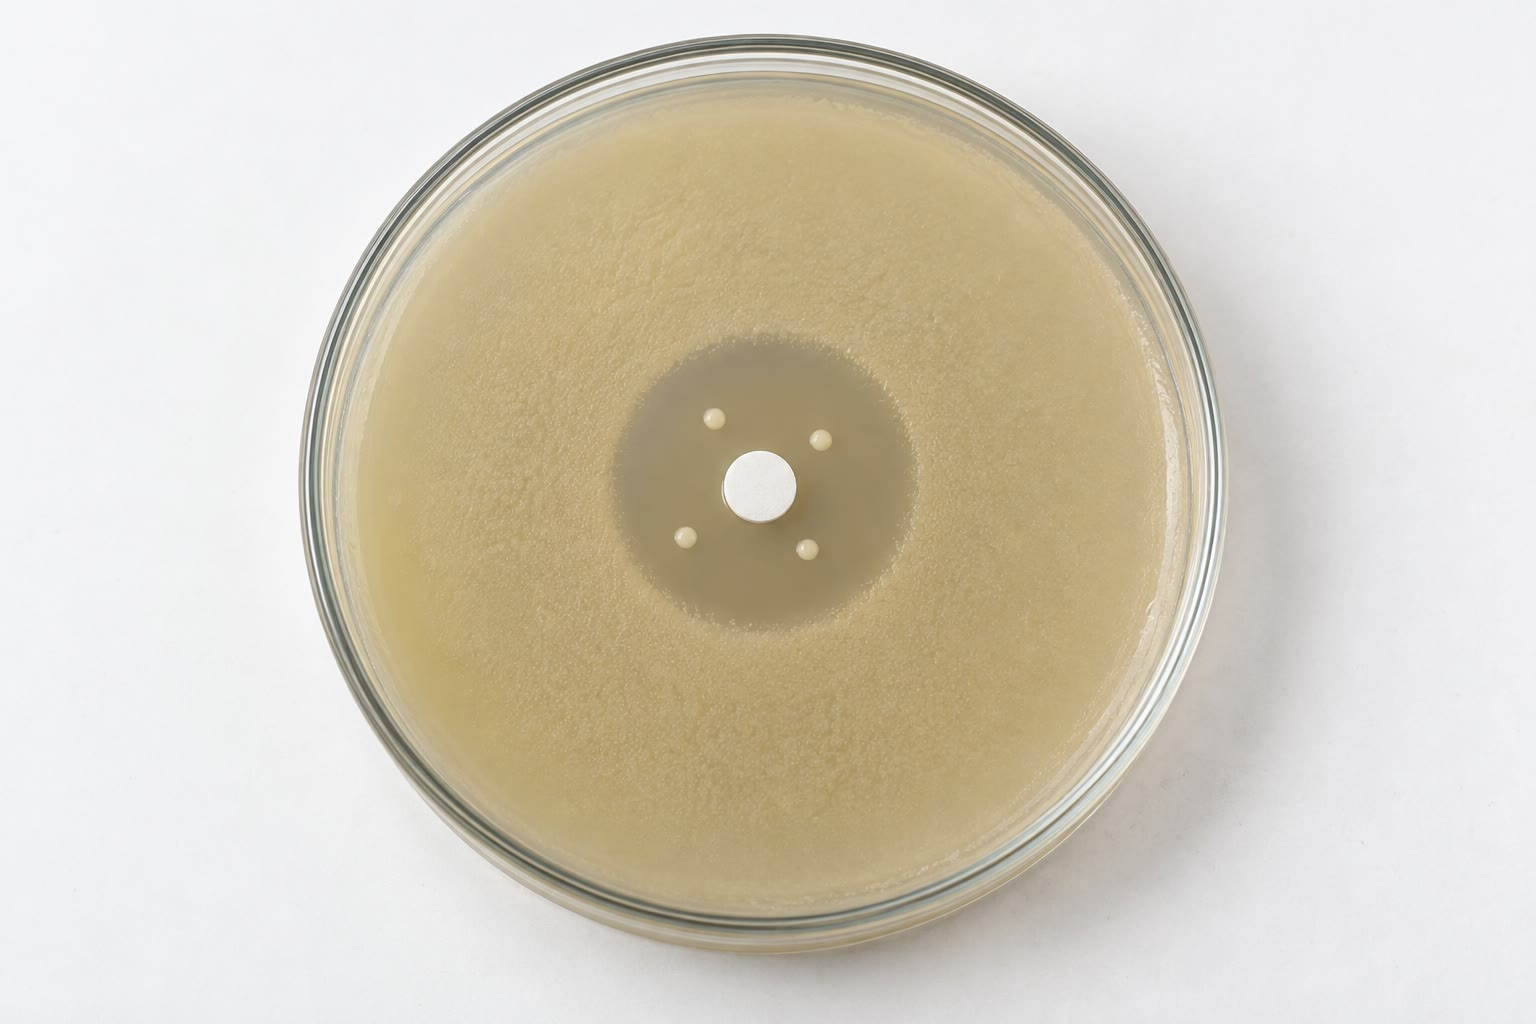
\includegraphics[width=0.5\linewidth]{images/book4/ai/b4-03-luria-plate.jpg}

{\small قرص صادّ على مرج من البكتيريا: المنطقة الصافية هي حيث قتل
الدواء المنتشر من القرص الخلايا الحساسة، والمستعمرات داخلها نمت من
طافرات مقاومة كانت موجودة قبل وضع القرص.}
\end{omfigure}

\begin{proposition}[الإصلاح وحدوده]\label{prop:b2:genome-diversification:repair}
\index{إصلاح DNA}
تصحح الخلية معظم الأذى قبل أن يصير \omterm{def:b2:genome-diversification:mutation}{طفرة}. أما \emph{\omterm{prop:b2:genome-diversification:repair}{إصلاح عدم التوافق}}
فيزيل الأساس الخطأ من السلسلة المصنوعة حديثًا. و\emph{إصلاح القطع
الأساسي} يقتطع أساسًا واحدًا متأذيًا (يوراسيل، أو غوانين مؤكسد)
ويملأ الفجوة؛ وهذا سبب استعمال DNA الثيمين بدل اليوراسيل: فاليوراسيل
في DNA لا يمكن أن يكون إلا سيتوزينًا منزوع الأمين، فيُعرف غريبًا.
و\emph{إصلاح القطع النوكليوتيدي} يزيل شريطًا من نحو اثني عشر أساسًا
حول أذى ضخم كثنائي الثيمين؛ ومن يفتقرون إليه (جفاف الجلد المصطبغ)
تنشأ عندهم سرطانات جلد من ضوء الشمس العادي. و\emph{إصلاح إعادة
التركيب} يعيد بناء صبغي مكسور من نسخته الشقيقة. وما يفلت من الإصلاح
أو يُصلح خطأً يصير \omterm{def:b2:genome-diversification:mutation}{طفرة} --- والخلية التي فقدت جملة إصلاح
(\emph{مطفِّرة}) تطفر أسرع بمئة مرة، وهذه ميزة قصيرة الأمد تحت
الإجهاد وعبء طويل الأمد. وتُعالَج آليات الإصلاح بتوسع في مجلد
السنة الثالثة.
\end{proposition}

\section{مورّثات تتحرك}

\begin{definition}[العناصر المنقولة]\label{def:b2:genome-diversification:transposon}
\index{قافزة}\index{قافزة راجعة}
\emph{العنصر المنقول} قطعة من DNA تستطيع الانتقال إلى موضع جديد في
المورثوم. و\emph{القافزات الدنوية} ترمّز \emph{ناقلة} تقتطع العنصر
وتلصقه في مكان آخر (أو تنسخه هناك)؛ وأبسطها متواليات الإقحام
البكتيرية (مورّثة ناقلة بين تكرارين مقلوبين)، أما القافزات المركبة
فتحمل مورّثات إضافية --- كثيرًا ما تكون مقاومات للصادات --- بين
اثنتين منها. و\emph{القافزات الراجعة} تنتقل بطريق النسخ واللصق عبر
وسيط من RNA، يُنسخ رجوعًا إلى DNA بمستنسخة عكسية؛ وهي لا تغادر
موضعها القديم أبدًا فتتراكم. والعنصر الذي يحط في مورّثة يعطلها؛ وإذا
حط قربها فقد يغير تعبيرها؛ ونسختان منه في صبغي واحد تتيحان مواضع
\omterm{prop:b2:genome-diversification:duplication}{لتعابر غير متساوٍ}. والقافزات وبقاياها تشكل نصف المورثوم البشري
وثمانين في المئة من مورثوم الذرة؛ ومعظمها اليوم غير متحرك.
\end{definition}
\begin{proof}[شواهد]
درست مكلينتوك (في الأربعينيات والخمسينيات) حبات ذرة فقدت صبغتها
الأرجوانية في بعض الخلايا واستعادتها في أخرى، فأعطت حبات مرقّطة.
وبيّنت بالتهجين وبمراقبة الصبغيات أن عدم الاستقرار سببه عنصر
(\emph{عنصر الانفصال} Ds) يكسر الصبغي حيث يجلس وينتقل بين المواضع تحت
سيطرة عنصر ثانٍ (\emph{عنصر التنشيط} Ac)، وأن المورّثة تُسكت حين يجلس
العنصر فيها وتُنشّط حين يغادرها. فالمورّثات، كما استنتجت، تستطيع
تغيير موضعها؛ ولم تُقبل الفكرة إلا بعد عشرين سنة، حين وُجدت متواليات
الإقحام البكتيرية، فنالت عليها جائزة نوبل سنة 1983.
\end{proof}

\begin{omfigure}
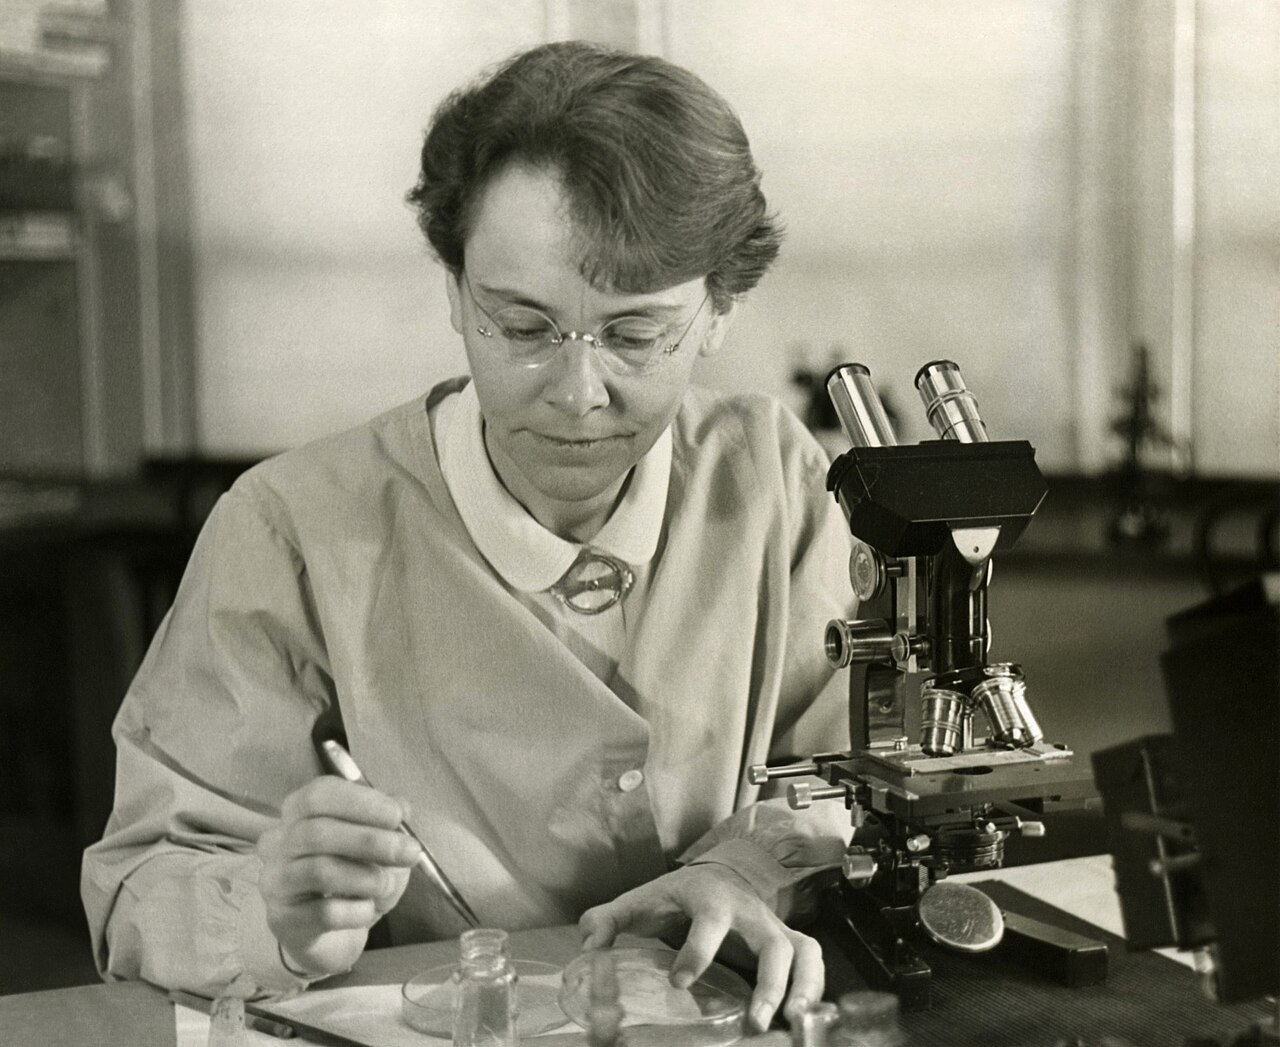
\includegraphics[width=0.4\linewidth]{images/book4/mcclintock.jpg}\hspace{0.04\linewidth}
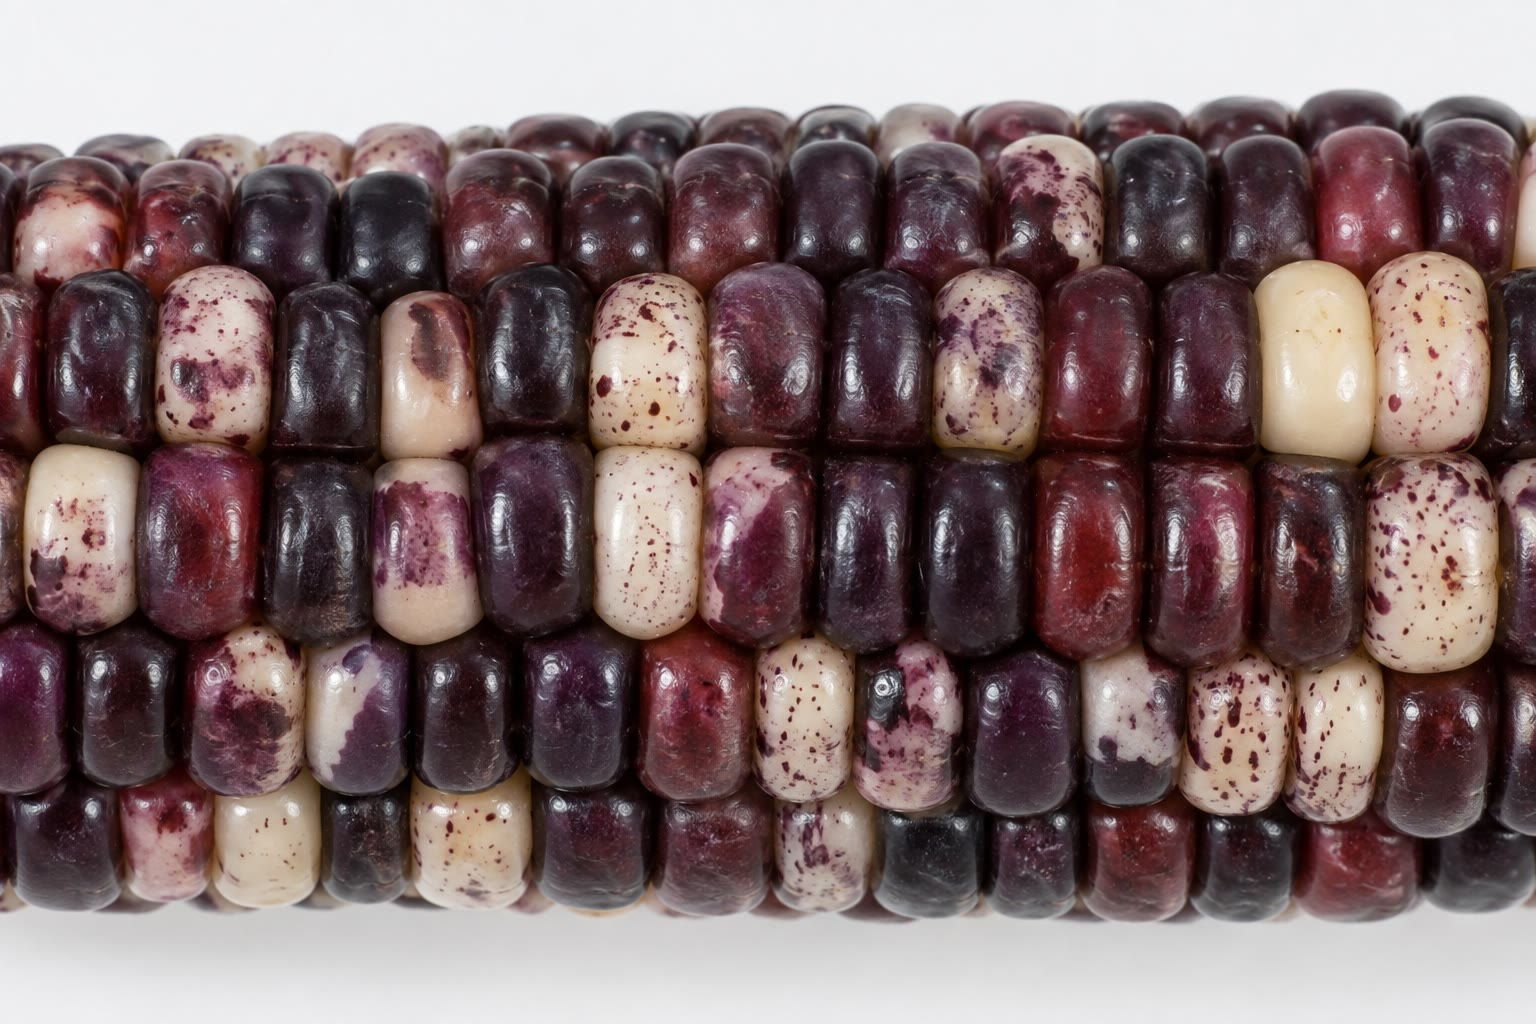
\includegraphics[width=0.5\linewidth]{images/book4/ai/b4-03-maize-kernels.jpg}

{\small باربرا مكلينتوك، والحبات التي قادتها إلى العناصر المنقولة:
مورّثة صبغة أرجوانية تُطفأ بعنصر مقحم ثم تُشعل من جديد، خلية خلية،
حين يقفز العنصر خارجًا، فيترك رقطًا وقطاعات.}
\end{omfigure}

\begin{omfigure}
\begin{tikzpicture}[every node/.style={font=\scriptsize}]
  % cut and paste
  \begin{scope}
    \draw[very thick, gray] (0,1.2) -- (4.5,1.2);
    \fill[omThm!70] (0.8,1.05) rectangle (1.8,1.35); \node[white, font=\tiny] at (1.3,1.2) {Tn};
    \draw[very thick, gray] (0,0) -- (4.5,0);
    \fill[omThm!70] (2.8,-0.15) rectangle (3.8,0.15); \node[white, font=\tiny] at (3.3,0) {Tn};
    \draw[->, thick, omThm] (1.3,1.0) .. controls (1.3,0.5) and (3.3,0.7) .. (3.3,0.2);
    \draw[dashed, gray] (0.8,1.2) -- (1.8,1.2);
    \node[align=center] at (2.25,-0.6) {قص ولصق (قافزة دنوية):\\العنصر يغادر موضعه القديم};
  \end{scope}
  % copy and paste
  \begin{scope}[xshift=7.5cm]
    \draw[very thick, gray] (0,1.2) -- (4.5,1.2);
    \fill[omProp!80] (0.8,1.05) rectangle (1.8,1.35); \node[white, font=\tiny] at (1.3,1.2) {RT};
    \draw[very thick, gray] (0,0) -- (4.5,0);
    \fill[omProp!80] (2.8,-0.15) rectangle (3.8,0.15); \node[white, font=\tiny] at (3.3,0) {RT};
    \draw[->, thick, omProp] (1.3,1.0) .. controls (1.3,0.5) and (3.3,0.7) .. (3.3,0.2);
    \node[omProp, anchor=west, align=left] at (3.6,0.75) {نسخة RNA،\\مستنسخة عكسيًا};
    \node[align=center] at (2.25,-0.6) {نسخ ولصق (قافزة راجعة):\\النسخة القديمة تبقى، والعدد ينمو};
  \end{scope}
\end{tikzpicture}

{\small طريقتان للانتقال. \omterm{def:b2:genome-diversification:transposon}{القافزة} الدنوية تُقتطع وتُعاد إقحامها؛
\omterm{def:b2:genome-diversification:transposon}{والقافزة الراجعة} تُستنسخ، ثم تُنسخ رجوعًا إلى DNA وتُقحم في مكان
آخر، فتتراكم نسخها.}
\end{omfigure}

\begin{definition}[النقل الأفقي للمورّثات]\label{def:b2:genome-diversification:hgt}
\index{نقل أفقي للمورّثات}\index{تحول}\index{اقتران!بكتيري}\index{نقل بالعاثيات}
تكتسب بدائيات النوى مورّثات من خلايا ليست أبويها بثلاثة طرق.
\emph{التحول}: تلتقط الخلية DNA عاريًا من محيطها (أطلقته خلايا
ميتة) وتعيد تركيبه في صبغيها؛ وبعض الأنواع كفؤة طبيعيًا، وهذا هو
الطريق الذي تتبادل به المكورات الرئوية مورّثات المحفظة.
و\emph{الاقتران}: يبني واهب يحمل بلازميدًا اقترانيًا (عامل F عند
\emph{E.~coli}) هلبًا، ويجذب متلقيًا إليه، ويمرر سلسلة مفردة من
\omterm{def:b2:unicellular-diversity:prokaryote}{البلازميد} عبر ثقب بينما ينسخها بطريقة الحلقة المتدحرجة؛ وإذا كان
\omterm{def:b2:unicellular-diversity:prokaryote}{البلازميد} قد اندمج في الصبغي (سلالة Hfr) انتقلت المورّثات الصبغية
بالترتيب خلفه، ورسم زمن دخول كل منها خريطة الصبغي.
و\emph{النقل بالعاثيات}: تحزم عاثية قطعة من DNA المضيف خطأً وتحقنها
في الخلية التالية التي تصيبها. وهذه الطرق مجتمعة تنقل مورّثات
المقاومة بين الأنواع داخل المستشفيات في سنوات، وقد نقلت مورّثات
استقلابية عبر الشجرة البكتيرية كلها على مدى الزمن الجيولوجي، حتى
صار نسب \omterm{def:b2:unicellular-diversity:prokaryote}{بدائي النواة} شبكة بقدر ما هو شجرة
(\cref{ch:b2:phylogenetic-trees}).
\end{definition}
\begin{proof}[شواهد]
خلط ليدربرغ وتاتوم (1946) سلالتين من \emph{E.~coli}، كل منهما عاجزة
عن صنع مغذيين مختلفين، وزرعا الخليط على وسط أدنى لا تستطيع أي منهما
النمو عليه وحدها: فظهرت مستعمرات، بنحو واحدة لكل عشرة ملايين خلية،
تستطيع صنع الأربعة جميعًا --- أي معاد تركيبها. ثم أعاد دايفيس (1950)
التجربة مع فصل السلالتين بمرشح يمرر الجزيئات دون الخلايا: فلم تظهر
معادات التركيب، أي إن التماس لازم. ثم بيّن هايز أن النقل أحادي
الاتجاه، من واهب إلى متلقٍّ، وقطع وولمان وجاكوب (1956) التزاوجات في
خلاط على فترات، فوجدا مورّثات الواهب تدخل المتلقي بترتيب ثابت، واحدة
إثر أخرى، على مدى نحو مئة دقيقة.
\end{proof}

\begin{omfigure}
\begin{minipage}[b]{0.56\linewidth}\centering
\begin{tikzpicture}[every node/.style={font=\scriptsize}]
  % donor
  \draw[thick, fill=omDef!8] (0,0) ellipse (1.5 and 0.75);
  \draw[thick, omDef] (0.2,0) circle (0.45);
  \draw[thick, omThm] (-0.9,0.1) circle (0.22);
  \node[anchor=south] at (0,1.25) {واهب $F^+$};
  \draw[omThm] (-0.9,-0.12) -- (-1.1,-1.0) node[below] {بلازميد F};
  \draw[omDef] (0.4,-0.4) -- (0.6,-1.0) node[below] {الصبغي};
  % recipient
  \draw[thick, fill=omDef!8] (5,0) ellipse (1.5 and 0.75);
  \draw[thick, omDef] (5.2,0) circle (0.45);
  \node[anchor=south] at (5,1.25) {متلقٍّ $F^-$};
  % pilus
  \draw[very thick, omThm] (1.5,0) -- (3.5,0);
  \node[omThm, below] at (2.5,-0.05) {هلب};
  % single strand transferred
  \draw[->, thick, omThm, dashed] (-0.7,0.15) .. controls (1.0,0.7) and (3.0,0.7) .. (4.1,0.4);
  \node[omThm, anchor=south] at (2.5,0.7) {سلسلة واحدة تُنسخ بالحلقة المتدحرجة};
  \draw[thick, omThm, dashed] (4.1,0.2) circle (0.2);
\end{tikzpicture}
\end{minipage}\hfill
\begin{minipage}[b]{0.42\linewidth}\centering
\begin{tikzpicture}
\begin{axis}[
  width=\linewidth, height=4.6cm,
  axis x line=bottom, axis y line=left,
  xmin=0, xmax=40, ymin=0, ymax=1.1,
  xlabel={دقائق قبل الخلط}, ylabel={معادات التركيب (نسبيًا)},
  xlabel style={font=\scriptsize, at={(axis description cs:0.5,-0.18)}, anchor=north},
  ylabel style={font=\scriptsize},
  tick label style={font=\scriptsize}, xtick={0,10,20,30,40}, ytick={0,0.5,1},
  legend style={font=\scriptsize, at={(0.97,0.08)}, anchor=south east, draw=none},
  clip=false,
]
\addplot[very thick, omDef, domain=8:40, samples=40] {1-exp(-(x-8)/5)};
\addlegendentry{\emph{thr}، تدخل عند \qty{8}{min}}
\addplot[very thick, omProp, domain=17:40, samples=40] {1-exp(-(x-17)/5)};
\addlegendentry{\emph{lac}، \qty{17}{min}}
\addplot[very thick, omThm, domain=25:40, samples=40] {1-exp(-(x-25)/5)};
\addlegendentry{\emph{gal}، \qty{25}{min}}
\end{axis}
\end{tikzpicture}
\end{minipage}

{\small على اليمين: الاقتران --- يمرر الواهب سلسلة واحدة من \omterm{def:b2:unicellular-diversity:prokaryote}{بلازميد}
F عبر وصلة الهلب بينما ينسخها. وعلى اليسار: تجربة التزاوج المقطوع
مع واهب Hfr: تبدأ كل مورّثة صبغية بالظهور بين معادات التركيب في زمن
مميز، وهو ما يرسم خريطة الصبغي بالدقائق.}
\end{omfigure}

\begin{omfigure}
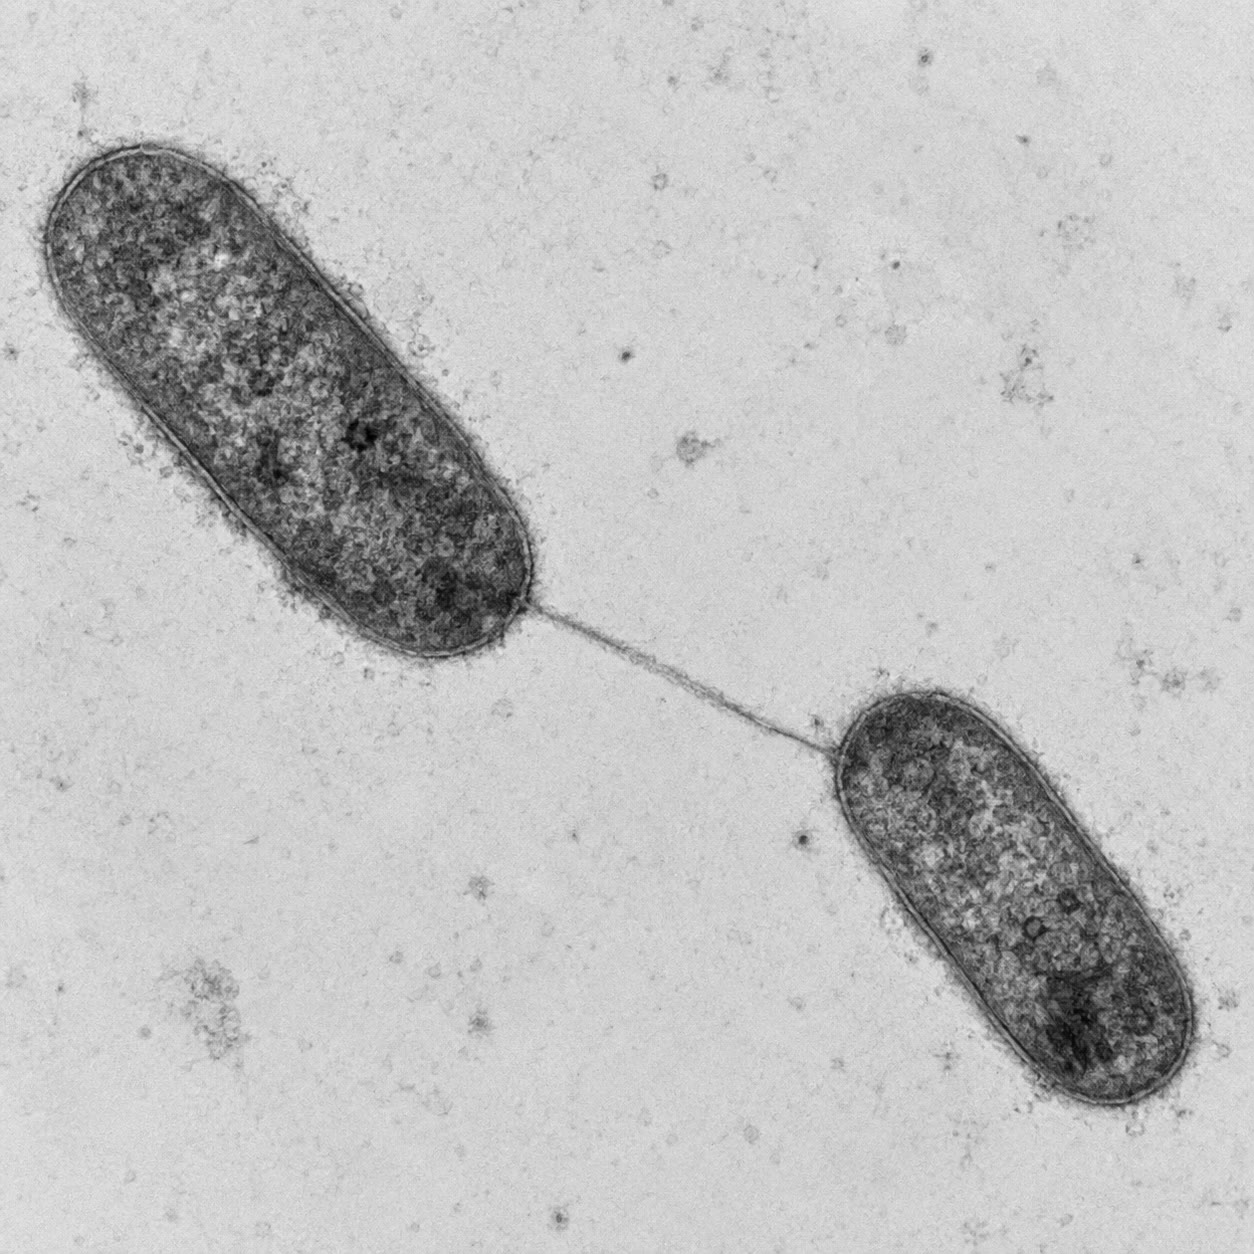
\includegraphics[width=0.42\linewidth]{images/book4/ai/b4-03-conjugation-tem.jpg}

{\small بكتيريتان موصولتان بهلب اقتراني، بالمجهر الإلكتروني
النافذ: الجسر الذي يمر عليه \omterm{def:b2:unicellular-diversity:prokaryote}{البلازميد}.}
\end{omfigure}

\begin{example}[المقاومة في حركة]\label{ex:b2:genome-diversification:resistance}
تنشأ مورّثة المقاومة عادةً مرة واحدة، \omterm{def:b2:genome-diversification:mutation}{بطفرة} أو من بكتيريا التربة
التي تصنع الصادّ، ثم تسافر: من صبغي إلى \omterm{def:b2:genome-diversification:transposon}{قافزة}، ومن \omterm{def:b2:genome-diversification:transposon}{القافزة} إلى
\omterm{def:b2:unicellular-diversity:prokaryote}{بلازميد} اقتراني، ومن \omterm{def:b2:unicellular-diversity:prokaryote}{البلازميد} عبر الأنواع بالاقتران وعبر السلالات
\omterm{def:b2:genome-diversification:hgt}{بالنقل بالعاثيات}، وعودًا إلى صبغي بالتحول. وقد وُجدت في اليابان في
الخمسينيات بلازميدات تحمل خمس مقاومات أو ستًا دفعة واحدة (مركّبة في
\emph{مدمجات} تأسر كاسيتات المورّثات)، بعد سنوات قليلة من دخول
الأدوية الاستعمال؛ ومورّثة الكاربابينيماز NDM-1، التي رئيت أول مرة
سنة 2008، بلغت كل قارة خلال ثلاث سنوات على \omterm{def:b2:unicellular-diversity:prokaryote}{بلازميد}. فتطور المقاومة
ليس في معظمه تطور مورّثات جديدة بل حركة مورّثات قديمة.
\end{example}

\section{المضاعفة: المورّثات والمورثومات}

\begin{proposition}[مضاعفة المورّثات وأسر المورّثات]\label{prop:b2:genome-diversification:duplication}
\index{مضاعفة مورّثية}\index{أسرة مورّثية}\index{تعابر غير متساوٍ}
حين يجلس تسلسلان متشابهان جنبًا إلى جنب على صبغي، قد يتزاوج
المتماثلان في غير موضعهما عند التقسم المنصّف ويتعابران تعابرًا غير
متساوٍ، فيحمل أحد الناتجين ثلاث نسخ والآخر نسخة واحدة. والمورّثة
المضاعفة زائدة عن الحاجة: فنسخة تستطيع الاحتفاظ بالعمل القديم بينما
تراكم الأخرى الطفرات بحرية --- فتتحلل عادةً إلى \emph{مورّثة كاذبة}،
وتكتسب أحيانًا وظيفة جديدة (\emph{تجديد الوظيفة}) أو نصيبًا من
القديمة (\emph{تجزئة الوظيفة}). وتكرار هذا على مدى مئات ملايين
السنين يبني \emph{أسر المورّثات}: الغلوبينات (فمورّثة سلفية واحدة
صارت الميوغلوبين، وعنقود $\alpha$، وعنقود $\beta$، بأفراد جنينية
وحملية وبالغة يُعبَّر عنها بالتناوب)، والمستقبلات الشمية (ألف مورّثة
عند فأر)، ومورّثات الصندوق المتماثل، وبلورينات العدسة. ومعظم مورّثات
المورثوم تنتمي إلى أسرة، والمضاعفة هي المصدر الرئيس للمورّثات
الجديدة.
\end{proposition}
\begin{proof}[شواهد]
يحوي عنقود $\beta$ غلوبين البشري على الصبغي 11 خمس مورّثات عاملة
($\varepsilon$، $^{G}\gamma$، $^{A}\gamma$،
$\delta$، $\beta$) ومورّثة كاذبة، بالترتيب الذي تُشعل به خلال النمو،
وكلها بالبنية نفسها من إكسونات وإنترونات، وتسلسلاتها أشد تشابهًا
كلما كان تباعدها أحدث؛ ولعنقود $\alpha$ على الصبغي 16 المعمار نفسه.
وحذف مورّثة $\alpha$ أو أكثر، الناتج عن \omterm{prop:b2:genome-diversification:duplication}{تعابر غير متساوٍ} بين النسخ
شبه المتطابقة، شائع ويسبب الثلاسيميا $\alpha$؛ والناتج المقابل، وهو
صبغي بثلاث مورّثات $\alpha$، موجود في الجمهرات نفسها.
\end{proof}

\begin{omfigure}
\begin{tikzpicture}[every node/.style={font=\scriptsize}]
  % unequal crossing over
  \begin{scope}
    \draw[very thick, gray] (0,1.2) -- (5,1.2);
    \fill[omDef!70] (1.0,1.05) rectangle (2.0,1.35); \fill[omDef!70] (2.4,1.05) rectangle (3.4,1.35);
    \draw[very thick, gray] (0,0) -- (5,0);
    \fill[omDef!70] (1.0,-0.15) rectangle (2.0,0.15); \fill[omDef!70] (2.4,-0.15) rectangle (3.4,0.15);
    \node[above] at (1.5,1.35) {A}; \node[above] at (2.9,1.35) {A$'$};
    \draw[very thick, omThm] (2.9,1.05) -- (1.5,0.15);
    \node[align=center] at (2.5,-0.6) {متماثلان متزاوجان في غير موضعهما\\يتعابران تعابرًا غير متساوٍ};
    \draw[->, thick, gray] (5.3,0.6) -- (6.1,0.6);
    % products
    \draw[very thick, gray] (6.5,1.2) -- (11.5,1.2);
    \fill[omDef!70] (7.5,1.05) rectangle (8.5,1.35); \fill[omDef!70] (8.9,1.05) rectangle (9.9,1.35); \fill[omDef!70] (10.3,1.05) rectangle (11.3,1.35);
    \node[above] at (9.4,1.35) {ثلاث نسخ};
    \draw[very thick, gray] (6.5,0) -- (11.5,0);
    \fill[omDef!70] (7.5,-0.15) rectangle (8.5,0.15);
    \node[above] at (8.0,0.15) {نسخة واحدة};
  \end{scope}
  % globin family tree
  \begin{scope}[yshift=-3.6cm]
    \draw[thick] (2,2.2) -- (2,1.7);
    \draw[thick] (0.5,1.7) -- (3.5,1.7);
    \draw[thick] (0.5,1.7) -- (0.5,0.4); \node[below] at (0.5,0.4) {ميوغلوبين};
    \draw[thick] (3.5,1.7) -- (3.5,1.2);
    \draw[thick] (2.3,1.2) -- (4.7,1.2);
    \draw[thick] (2.3,1.2) -- (2.3,0.4); \node[below] at (2.3,0.4) {أسرة $\alpha$};
    \draw[thick] (4.7,1.2) -- (4.7,0.9);
    \draw[thick] (3.6,0.9) -- (5.8,0.9);
    \draw[thick] (3.6,0.9) -- (3.6,0.4); \node[below] at (3.6,0.4) {$\varepsilon,\gamma$};
    \draw[thick] (5.8,0.9) -- (5.8,0.7);
    \draw[thick] (5.2,0.7) -- (6.4,0.7);
    \draw[thick] (5.2,0.7) -- (5.2,0.4); \node[below] at (5.2,0.4) {$\delta$};
    \draw[thick] (6.4,0.7) -- (6.4,0.4); \node[below] at (6.4,0.4) {$\beta$};
    \node[anchor=west, align=left] at (7.2,1.7) {مضاعفات لمورّثة غلوبين سلفية واحدة:\\قبل الفقاريات (ميوغلوبين/هيموغلوبين)،\\قبل $\sim$450 مليون سنة ($\alpha$/$\beta$)،\\ثم داخل عنقود $\beta$ (جنينية، وحملية، وبالغة)};
    \node[anchor=east, gray] at (1.9,2.1) {غلوبين سلفي};
  \end{scope}
\end{tikzpicture}

{\small في الأعلى: التعابر غير المتساوي بين نسختين متجاورتين
متزاوجتين في غير موضعهما يعطي صبغيًا بثلاث نسخ وآخر بنسخة واحدة.
وفي الأسفل: أسرة الغلوبينات، مبنية بمضاعفات وتباعدات متعاقبة.}
\end{omfigure}

\begin{definition}[تعدد الصيغة الصبغية]\label{def:b2:genome-diversification:polyploidy}
\index{تعدد الصيغة الصبغية}\index{تعدد صيغة مغاير}\index{تعدد صيغة ذاتي}
\emph{متعدد الصيغة الصبغية} يحمل أكثر من طقمين كاملين من الصبغيات.
و\emph{متعدد الصيغة الذاتي} له عدة طقوم من نوع واحد (فتقسم منصّف
فاشل يعطي عروسًا ثنائية الصيغة؛ وعروسان كهاتين تعطيان رباعي صيغة)؛
أما \emph{متعدد الصيغة المغاير} فيجمع طقمي نوعين بعد تهجين. والهجين
الثنائي الصيغة AB، وليس لأي صبغي فيه متماثل، لا يستطيع تزويج صبغياته
عند التقسم المنصّف فيكون عقيمًا؛ فإذا تضاعف مورثومه إلى AABB صار لكل
صبغي شريك من جديد، وعمل التقسم المنصّف، وصار النبات الجديد خصيبًا
--- لكنه لا يستطيع التهجين الرجعي مع أي من الأبوين (فالخلف AAB
عقيم). وهكذا يصنع تعدد الصيغة نوعًا جديدًا في خطوة واحدة، ونحو ثلث
أنواع النباتات الزهرية نشأ هكذا: فقمح الخبز سداسي صيغة AABBDD من
ثلاث نجيليات، وفراولة الحديقة ثمانية الصيغة، والقطن والتبغ رباعيا
صيغة مغايران، وسلالة الفقاريات نفسها ضاعفت مورثومها مرتين قرب
نشأتها. ومتعددات الصيغة أكبر عادةً من أسلافها الثنائية الصيغة (فدنا
أكثر، وخلايا أكبر) ويعزّها المربّون كثيرًا.
\end{definition}

\begin{omfigure}
\begin{tikzpicture}[every node/.style={font=\scriptsize}]
  \node[draw, rounded corners, fill=omDef!10, align=center] (a) at (0,0) {\emph{T.~urartu}\\AA, $2n = 14$};
  \node[draw, rounded corners, fill=omDef!10, align=center] (b) at (3.4,0) {\emph{Aegilops}\\BB, $2n = 14$};
  \node[draw, rounded corners, fill=omProp!15, align=center] (ab) at (1.7,-1.5) {هجين AB\\$n = 14$، عقيم};
  \node[draw, rounded corners, fill=omExo!25, align=center] (aabb) at (1.7,-3.1) {قمح الإمر AABB\\$2n = 28$، خصيب};
  \node[draw, rounded corners, fill=omDef!10, align=center] (d) at (6.4,-3.1) {\emph{Ae.~tauschii}\\DD, $2n = 14$};
  \node[draw, rounded corners, fill=omProp!15, align=center] (abd) at (4.0,-4.6) {هجين ABD\\$3n = 21$، عقيم};
  \node[draw, rounded corners, fill=omExo!25, align=center] (abd2) at (4.0,-6.1) {قمح الخبز AABBDD\\$2n = 42$، خصيب};
  \draw[->, thick] (a) -- (ab); \draw[->, thick] (b) -- (ab);
  \draw[->, thick] (ab) -- (aabb) node[midway, right] {مضاعفة المورثوم};
  \draw[->, thick] (aabb) -- (abd); \draw[->, thick] (d) -- (abd);
  \draw[->, thick] (abd) -- (abd2) node[midway, right] {مضاعفة المورثوم};
  \node[anchor=west, align=left, gray] at (7.8,-1.5) {كل تهجين يعطي نباتًا عقيمًا\\بصبغيات غير متزاوجة؛\\وكل مضاعفة تعيد التزاوج\\والخصوبة --- وتصنع نوعًا\\لا يستطيع التهجين الرجعي};
\end{tikzpicture}

{\small نشأة قمح الخبز: تهجينان، تلا كلًا منهما مضاعفة للمورثوم،
بنيا سداسي صيغة من ثلاث نجيليات ثنائية الصيغة في نحو عشرة آلاف سنة.}
\end{omfigure}

\begin{omfigure}
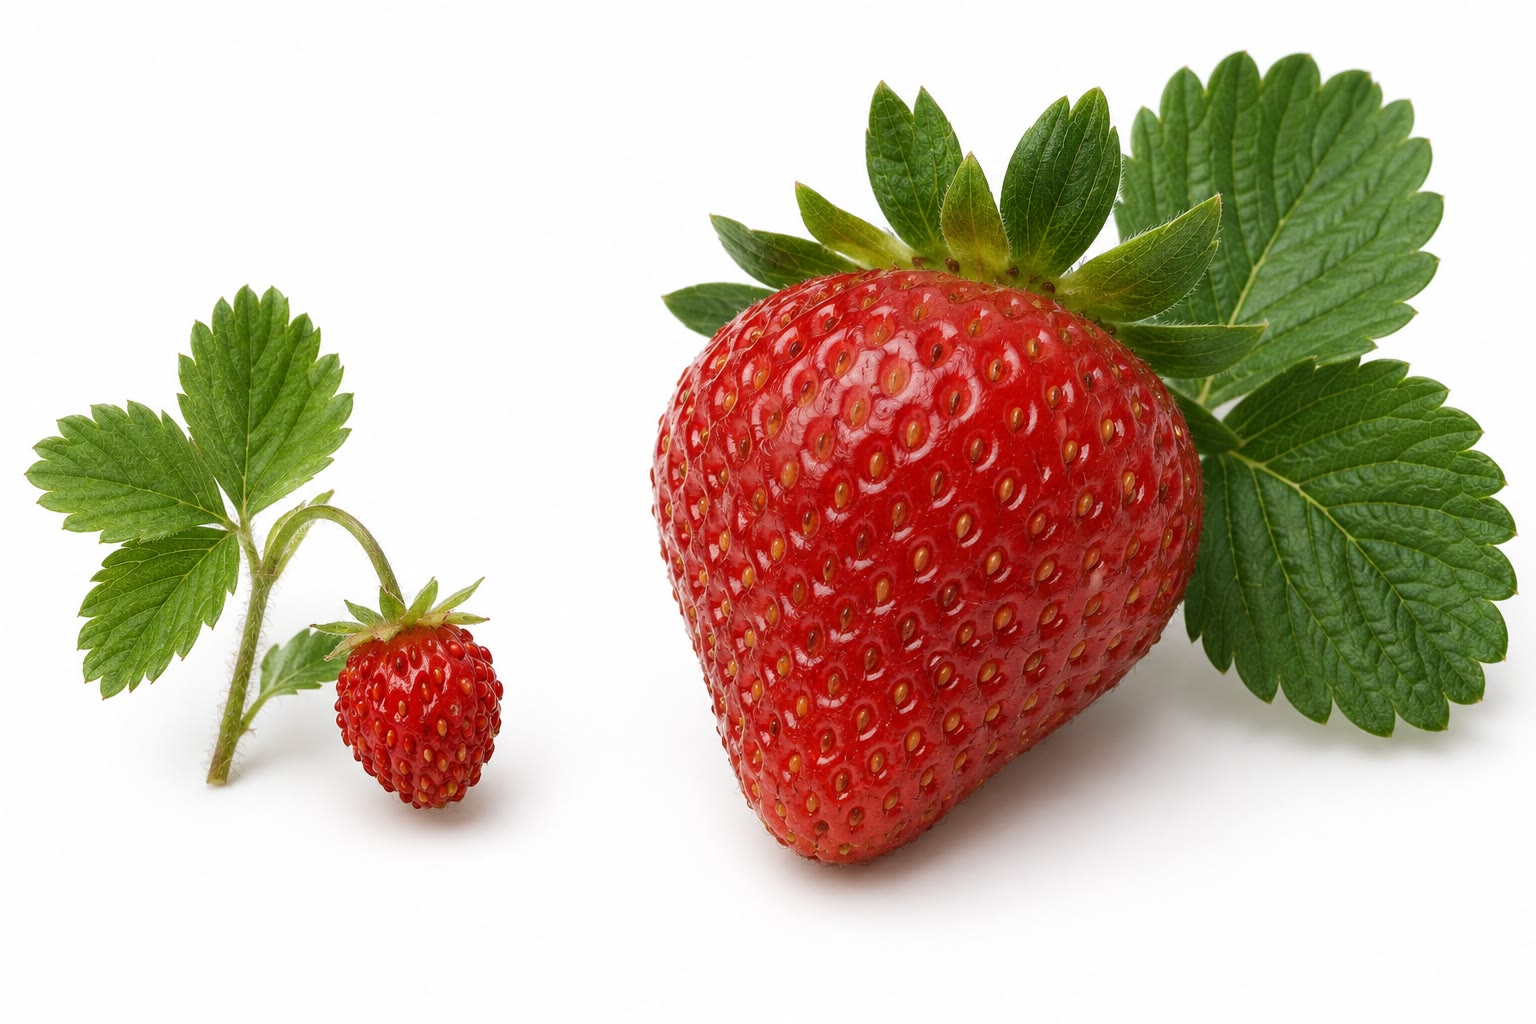
\includegraphics[width=0.55\linewidth]{images/book4/ai/b4-03-polyploid-strawberries.jpg}

{\small فراولة برية ثنائية الصيغة والفراولة المزروعة ثمانية الصيغة:
فمتعدد الصيغة، وفيه أربعة أضعاف DNA في كل خلية، هو النبات الأكبر
ذو الثمرة الأكبر.}
\end{omfigure}

\section{العشوائية والمعدل}

\begin{proposition}[الطفرة عشوائية بالنسبة إلى الحاجة]\label{prop:b2:genome-diversification:random}
\index{طفرة!عشوائيتها}
يبين \omterm{thm:b2:genome-diversification:luria}{اختبار التذبذب} والزرع بالنسخ أن \omterm{def:b2:genome-diversification:mutation}{الطفرة} النافعة في محيط جديد
تنشأ بالمعدل نفسه سواء أكان ذلك المحيط حاضرًا أم لا: فالمحيط ينتخب
بين الطفرات، ولا يستدعيها. \omterm{def:b2:genome-diversification:mutation}{والطفرة} ليست عشوائية بكل معنى ---
فالانتقالات أكثر من التحويلات، وثنائيات النوكليوتيد CpG تطفر أسرع
بعشر مرات من سواها (إذ ينزع الأمين من سيتوزينها المُمثيل فيصير
ثيمينًا لا يعرفه الإصلاح غريبًا)، وبعض المناطق بؤر ساخنة، والإجهاد
يستطيع رفع المعدل العام --- لكنها عمياء عن العواقب. \omterm{thm:b2:genome-diversification:rate}{ومعدل الطفر}
نفسه صفة موروثة، والانتخاب يعايره: فإن علا ورث كل جيل تغيرات ضارة؛
وإن هبط عجزت الجمهرة عن مجاراة عالم متغير. فالسلالات المطفِّرة تربح
قليلًا في مستشفى وتخسر على المدى الطويل، والمعدل $10^{-9}$ لكل أساس
الذي تستقر عليه معظم الخلايا حل وسط بين كلفة الأخطاء وكلفة التدقيق.
\end{proposition}

\section{تمارين}

\begin{exercise}[$\star$]\label{exo:b2:genome-diversification:1}
صنّف كل تغير يصيب الرامزة GAA (غلوتامات): GAG؛ وGTA؛ وTAA؛ وإقحام
C بعد الأساس الأول. وأيها انتقال وأيها تحويل؟
\end{exercise}

\begin{exercise}[$\star$]\label{exo:b2:genome-diversification:2}
مع $u = \qty{5e-10}{}$ لكل زوج أسس في النسخة الواحدة و$G =
\qty{4.6e6}{}$، كم \omterm{def:b2:genome-diversification:mutation}{طفرة} جديدة ينتج انقسام واحد عند \emph{E.~coli}
وسطيًا؟ وكم في الجيل في مزرعة من
$10^{9}$ خلية؟
\end{exercise}

\begin{exercise}[$\star$]\label{exo:b2:genome-diversification:3}
سمِّ طرق \omterm{def:b2:genome-diversification:hgt}{النقل الأفقي للمورّثات} الثلاثة، وقل في كل منها ما يلزمه
(تماس، أو فيروس، أو DNA حر) وما ينقله عادةً.
\end{exercise}

\begin{exercise}[$\star$]\label{exo:b2:genome-diversification:4}
ميّز \omterm{def:b2:genome-diversification:polyploidy}{تعدد الصيغة الذاتي} من \omterm{def:b2:genome-diversification:polyploidy}{تعدد الصيغة المغاير}، بمثال على كل منهما،
واشرح لماذا يكون الهجين الثنائي الصيغة بين نوعين عقيمًا عادةً.
\end{exercise}

\begin{exercise}[$\star\star$]\label{exo:b2:genome-diversification:5}
تراكم سلالة جنسية بشرية $u = \qty{1.2e-8}{}$ \omterm{def:b2:genome-diversification:mutation}{طفرة} لكل زوج أسس في
الجيل على مورثوم فردي من \qty{3.2e9}{} زوج أسس. فكم \omterm{def:b2:genome-diversification:mutation}{طفرة} جديدة يحمل
الطفل؟ وإذا كانت \qty{1.5}{\%} من المورثوم ترمّز البروتين وكانت
\qty{70}{\%} من الاستبدالات المرمّزة تغير حمضًا أمينيًا، فكم تغيرًا
جديدًا في الحموض الأمينية يحمل الطفل؟
\end{exercise}

\begin{exercise}[$\star\star$]\label{exo:b2:genome-diversification:6}
تنمو مزرعة من $10^{3}$ إلى $10^{9}$ خلية؛ وتقع \omterm{def:b2:genome-diversification:mutation}{طفرة} معينة عند
$m = \qty{2e-8}{}$ في الانقسام. احسب العدد المنتظر لأحداث الطفر
وللخلايا الطافرة. ولماذا يكون كسر المزارع الخالية من الطافرات عديم
الفائدة هنا لقياس $m$، وأي قياس مزرعة يجعله مفيدًا؟
\end{exercise}

\begin{exercise}[$\star\star$]\label{exo:b2:genome-diversification:7}
ينزع الأمين من السيتوزين فيصير يوراسيل؛ وينزع من 5-ميثيل سيتوزين
فيصير ثيمينًا. اشرح لماذا يُصلح الأول بكفاءة ولا يُصلح الثاني،
واستنتج لماذا تكون مواقع CpG (حيث يكون السيتوزين مُمثيلًا) بؤرًا
ساخنة للطفر وأندر في المورثوم مما تتنبأ به المصادفة.
\end{exercise}

\begin{exercise}[$\star\star$]\label{exo:b2:genome-diversification:8}
في تجربة تزاوج مقطوع، تدخل أربع مورّثات المتلقيَ عند 8 و17 و25
و\qty{40}{min}؛ والصبغي كله (\qty{4.6}{Mb}) يستغرق \qty{100}{min}.
حوّل الأزمنة إلى مواضع بالكيلوأساس واحسب المسافات بين المورّثات
المتتالية.
\end{exercise}

\begin{exercise}[$\star\star$]\label{exo:b2:genome-diversification:9}
ارسم التزاوج والتعابر الذي يحول صبغيين لكل منهما مورّثتا $\alpha$
غلوبين متجاورتان إلى صبغي بثلاث وآخر بواحدة. وشخص ورث صبغيًا ذا
مورّثة واحدة من كل من أبويه: فكم مورّثة $\alpha$ عنده، وماذا يُنتظر من
هيموغلوبينه؟
\end{exercise}

\begin{exercise}[$\star\star\star$]\label{exo:b2:genome-diversification:10}
قمح الخبز AABBDD مع $2n = 42$. أعط عدد صبغيات أعراسه، وعدد صبغيات
الهجن العقيمة في كل خطوة من نشأته، وعدد صبغيات تهجين بين قمح الخبز
وقمح الإمر (AABB). واشرح بدلالة التزاوج المنصّف لماذا أعادت كل
مضاعفة الخصوبة ولماذا لا يستطيع سداسي الصيغة التهجين الرجعي مع
أبويه.
\end{exercise}

\begin{exercise}[$\star\star\star$]\label{exo:b2:genome-diversification:11}
في جمهرة معوية من $N = 10^{9}$ بكتيريا، ينتشر \omterm{def:b2:unicellular-diversity:prokaryote}{بلازميد} مقاومة
بالاقتران بمعدل يتناسب مع اللقاءات بين الحاملات $R$ وغير الحاملات
$N - R$: $\mathrm{d}R/\mathrm{d}t =
\gamma R (N - R)$ مع $\gamma N = \qty{0.5}{h^{-1}}$. حلّ المعادلة
انطلاقًا من حاملة واحدة، واحسب الزمن اللازم لأن يحمل \omterm{def:b2:unicellular-diversity:prokaryote}{البلازميد} نصف
الجمهرة. وماذا يحدث إذا سُحب الصادّ عندئذ وكان \omterm{def:b2:unicellular-diversity:prokaryote}{البلازميد} يكلف مضيفه
\qty{5}{\%} من معدل نموه؟
\end{exercise}

\begin{exercise}[$\star\star\star$]\label{exo:b2:genome-diversification:12}
«\omterm{def:b2:genome-diversification:mutation}{الطفرة} عشوائية؛ والتطور ليس كذلك.» ناقش هذا باستعمال \omterm{thm:b2:genome-diversification:luria}{اختبار
التذبذب}، والزرع بالنسخ، وكون \omterm{thm:b2:genome-diversification:rate}{معدل الطفر} نفسه خاضعًا للانتخاب.
\end{exercise}

\section{مسألة: اختبار تذبذب}

\begin{problem}[{مسألة نهاية الأسبوع --- يُجرى اختبار تذبذب ويُحلَّل،
ويُستخرج منه معدل طفر سلالة ويُقاس على مورثومها وجمهرتها، ويُنمذَج
انتشار بلازميد مقاومة، وتُوزن كلفة سلالة مطفِّرة، وتنتهي إلى معدل
طفر السلالة لكل أساس وزمن استيلاء البلازميد}]
\label{pb:b2:genome-diversification:1}
تُبدأ عشرون مزرعة من \emph{E.~coli}، كل منها من \num{100} خلية في
\qty{0.2}{mL}، وتُنمّى إلى $N = \qty{2e8}{}$ خلية؛ ثم تُنثر كل منها
على طبق مع عاثية، وتُعدّ المستعمرات المقاومة: 0، 0، 0، 1، 0، 0، 3،
0، 0، 1، 0، 0، 0، 0، 107، 0، 2، 0، 0، 5. وفي الوقت نفسه تُؤخذ عشرون
عينة من \qty{0.2}{mL} من مزرعة كبيرة واحدة بالكثافة نفسها وتُزرع
كذلك: 14، 15، 13، 21، 15، 14، 26، 16، 20، 13، 17، 12، 18، 14، 16،
19، 15، 13، 17، 16. والمورثوم: \qty{4.6e6}{} زوج أسس، \qty{88}{\%}
منها مرمّز. ويمكن أن تنشأ المقاومة للعاثية بأي واحد من \num{20}
تغيرًا مفردًا متميزًا في أساس واحد من مورّثة مستقبل واحدة.

\medskip
\noindent\textbf{الجزء الأول --- الاختبار.}
\begin{enumerate}
  \item احسب متوسط المزارع العشرين المستقلة وتباينها.
  \item احسب متوسط العينات العشرين وتباينها.
  \item في توزيع بواسون يساوي التباين المتوسط. فأي المجموعتين
        بواسونية، وماذا يقول توزيع كل منهما عن \emph{متى} وقعت
        الطفرات؟
  \item فسّر العدد 107.
  \item كم مزرعة من المستقلة لا تحوي طافرة؟ استعمل
        $p_0 = e^{-m(N - N_0)}$ لتقدير $m$، أي \omterm{thm:b2:genome-diversification:rate}{معدل الطفر} إلى
        المقاومة في الانقسام الخلوي الواحد.
  \item احسب العدد المنتظر للخلايا الطافرة في المزرعة من
        $mN\ln(N/N_0)$ وقارنه بالمتوسط المرصود.
  \item لماذا كانت عينات المزرعة الواحدة عديمة الفائدة لتقدير $m$
        بطريقة $p_0$؟
\end{enumerate}

\medskip
\noindent\textbf{الجزء الثاني --- القياس على المورثوم.}
\begin{enumerate}[resume]
  \item استنتج \omterm{thm:b2:genome-diversification:rate}{معدل الطفر} $u$ لكل زوج أسس في النسخة الواحدة من $m$
        ومن عدد التغيرات المانحة للمقاومة.
  \item احسب العدد الوسطي للطفرات الجديدة في المورثوم في النسخة
        الواحدة، $U$.
  \item مزرعة من لتر واحد عند $10^{9}$ خلية في المليلتر تتضاعف مرة
        واحدة. فكم \omterm{def:b2:genome-diversification:mutation}{طفرة} جديدة تنشأ في الجمهرة؟
  \item كم تغيرًا مفردًا متميزًا في أساس واحد ممكن في هذا المورثوم؟
        وكم مرة ينشأ كل منها وسطيًا في تلك المضاعفة الواحدة؟
  \item اشرح لماذا تكون المقاومة، في جمهرة كهذه، لأي صادّ منفرد
        تهزمه \omterm{def:b2:genome-diversification:mutation}{طفرة} واحدة مضمونة الحضور عمليًا.
  \item اشرح لماذا يغير الجمع بين صادّين يحتاجان إلى طفرتين
        مستقلتين هذا الأمر، مع رقم.
\end{enumerate}

\medskip
\noindent\textbf{الجزء الثالث --- انتشار \omterm{def:b2:unicellular-diversity:prokaryote}{بلازميد}.}
في أمعاء تضم $N = 10^{9}$ خلية، تكتسب خلية واحدة \omterm{def:b2:unicellular-diversity:prokaryote}{بلازميد} مقاومة
اقترانيًا. وتنقله الحاملات $R$ عند التماس:
$\mathrm{d}R/\mathrm{d}t = \gamma R(N - R)$، مع $\gamma N =
\qty{0.5}{h^{-1}}$.
\begin{enumerate}[resume]
  \item بيّن أن $R(t) = N/\bigl(1 + (N - 1)e^{-\gamma N t}\bigr)$
        يحقق المعادلة مع $R(0) = 1$.
  \item احسب الزمن الذي يحمل عنده نصف الخلايا \omterm{def:b2:unicellular-diversity:prokaryote}{البلازميد}.
  \item احسب الزمن الذي تحمله عنده \qty{99}{\%} منها.
  \item كم حدث اقتران يقع في الساعة لحظةَ يكون نصف الخلايا حاملًا؟
  \item قارن بالزمن اللازم لأن تبلغ \emph{طافرة} مقاومة نصف الجمهرة
        بنموها أسرع من البقية بنسبة \qty{10}{\%} تحت الصادّ (وزمن جيل
        الخلايا الحساسة \qty{1}{h}): فانطلاقًا من خلية واحدة، كم
        يستغرق ذلك؟
  \item استنتج لماذا تنتشر المقاومة بالنقل أساسًا لا بالتناسل.
\end{enumerate}

\medskip
\noindent\textbf{الجزء الرابع --- سلالة مطفِّرة.}
سلالة تفتقر إلى \omterm{prop:b2:genome-diversification:repair}{إصلاح عدم التوافق} تطفر أسرع بمقدار \num{100} مرة.
افترض أن \qty{30}{\%} من الطفرات في التسلسل المرمّز ضارة.
\begin{enumerate}[resume]
  \item احسب $U$ عندها والعدد الوسطي للطفرات الضارة في الخلية في
        الجيل.
  \item بعد \num{200} جيل، ما كسر ذرية سلالة لا يحمل أي \omterm{def:b2:genome-diversification:mutation}{طفرة} ضارة
        البتة (بواسون)؟
  \item احسب الشيء نفسه عند النمط البري.
  \item في \omterm{thm:b2:genome-diversification:luria}{اختبار التذبذب} أعلاه، أي متوسط عدد كانت المطفِّرة
        ستعطيه، وأي كسر من المزارع بلا طافرة؟
  \item اشرح في جملتين لماذا توجد السلالات المطفِّرة بين عزلات
        المستشفيات وتندر في الطبيعة.
  \item اذكر النتيجة: $m$ و$u$ و$U$ للسلالة، والزمنين اللذين يبلغ
        فيهما \omterm{def:b2:unicellular-diversity:prokaryote}{البلازميد} نصف الأمعاء و\qty{99}{\%} منها.
\end{enumerate}
\end{problem}
